\begin{abox}
	Statistical Mechanics 
	\end{abox}
\begin{enumerate}
	\item The Hamiltonian of a system of 3 spins is $H=J\left(S_{1} S_{2}+S_{2} S_{3}\right)$, where $S_{i}=\pm 1$ for $i=1,2,3$. Its canonical partition function, at temperature $T$, is
	{\exyear{NET/JRF(JUNE-2020)}}
\begin{tasks}(2)
\task[\textbf{A.}] $2\left(2 \sinh \frac{J}{k_{B} T}\right)^{2}$
\task[\textbf{B.}]  $2\left(2 \cosh \frac{J}{k_{B} T}\right)^{2}$
\task[\textbf{C.}]  $2\left(2 \cosh \frac{J}{k_{B} T}\right)$
\task[\textbf{D.}] $2\left(2 \cosh \frac{J}{k_{B} T}\right)^{3}$
\end{tasks}
\begin{answer}
\begin{align*}
\renewcommand*{\arraystretch}{1.5}
\begin{tabular}{|c|c|c|c|}
\hline$S_{1}$ & $S_{2}$ & $S_{3}$ & $H$ \\
\hline 1 & 1 & 1 & $2 \mathrm{~J}$ \\
\hline 1 & 1 & $-1$ & 0 \\
\hline 1 & $-1$ & 1 & 0 \\
\hline 1 & $-1$ & $-1$ & $-2 \mathrm{~J}$ \\
\hline$-1$ & 1 & 1 & 0 \\
\hline$-1$ & 1 & $-1$ & $-2 \mathrm{~J}$ \\
\hline$-1$ & $-1$ & 1 & 0 \\
\hline$-1$ & $-1$ & $-1$ & $2 \mathrm{~J}$ \\
\hline
\end{tabular}\\
\text{Number of states }2^{3}&=8\\
\end{align*}
\begin{align*}
H&=J\left(S_{1} S_{2}+S_{2} S_{3}\right)\\
Z&=2 e^{-\beta 2 J}+2 e^{\beta 2 J}+4=2\left[e^{\beta 2 J}+e^{-\beta 2 J}\right]+4\\&=2\left(\left[e^{\beta J}+e^{-\beta J}\right]^{2}-2\right)+4\\
\Rightarrow Z&=2\left(\frac{2\left(e^{\beta J}+e^{-\beta J}\right)}{2}\right)^{2}=2\left(2 \cosh \frac{J}{k_{B} T}\right)^{2}
\end{align*}
So the correct answer is \textbf{Option (B)}
\end{answer}
	\item The Hamiltonian of a classical nonlinear one dimensional oscillator is $H=\frac{1}{2 m} p^{2}+\lambda x^{4}$, where $\lambda>0$ is a constant. The specific heat of a collection of a collection of $N$ independent such oscillators is
{	\exyear{NET/JRF(JUNE-2019)}}
\begin{tasks}(4)
\task[\textbf{A.}] $\frac{3 N k_{B}}{2}$
\task[\textbf{B.}] $\frac{3 N k_{B}}{4}$
\task[\textbf{C.}] $N k_{B}$
\task[\textbf{D.}] $\frac{N k_{B}}{2}$
\end{tasks}
\begin{answer}
\begin{align*}
H&=\frac{p^{2}}{2 m}+\lambda x^{4}, \quad \lambda>0\\
\langle H\rangle&=\left\langle\frac{p^{2}}{2 m}\right\rangle+\langle V\rangle=\frac{1}{2} k_{B} T+2 \lambda \frac{\int_{0}^{\infty} x^{4} e^{-\beta x x^{4}} d x}{2 \int_{0}^{\infty} e^{-\beta x^{4}} d x}\\&=\frac{1}{2} k_{B} T+2 \lambda \frac{\frac{5 / 4}{4(\lambda \beta)^{5 / 4}}}{2 \frac{\sqrt{5 / 4}}{(\lambda \beta)^{1 / 4}}}\\
\Rightarrow\langle H\rangle&=\frac{1}{2} k_{B} T+\lambda \frac{(\lambda \beta)^{1 / 4}}{4(\lambda \beta)^{5 / 4}}=\frac{1}{2} k_{B} T+\frac{\lambda}{4} \frac{1}{\lambda \beta}=\frac{1}{2} k_{B} T+\frac{k_{B} T}{4}\\&=\frac{3}{4} k_{B} T=\frac{3}{4} k_{B} T\\
\Rightarrow C_{V}&=\frac{3}{4} N k_{B}
\end{align*}
So the correct answer is \textbf{Option (B)}
\end{answer}
	\item In a system comprising of approximately $10^{23}$ distinguishable particles, each particle may occupy any of 20 distinct states. The maximum value of the entropy per particle is nearest to
{	\exyear{NET/JRF(JUNE-2019)}}
\begin{tasks}(4)
\task[\textbf{A.}] $20 k_{B}$
\task[\textbf{B.}]  $3 k_{B}$
\task[\textbf{C.}] $10(\ln 2) k_{B}$
\task[\textbf{D.}] $20(\ln 2) k_{B}$
\end{tasks}
\begin{answer}
\begin{align*}
\text{	For $N$ particles; }\omega&=20^{N} .\\
S&=k_{B} \ln \omega=k_{B} \ln 20^{N}=N k_{B} \ln 20 \Rightarrow \frac{S}{N}\\&=k_{B} \ln 20 \approx 3 k_{B} \quad \because \ln 20 \approx 3
\end{align*}
So the correct answer is \textbf{Option (B)}
\end{answer}
	\item A particle hops on a one-dimensional lattice with lattice spacing $a$. The probability of the particle to hop to the neighboring site to its right is $p$, while the corresponding probability to hop to the left is $q=1-p$. The root-mean squared deviation $\Delta x=\sqrt{\left\langle x^{2}\right\rangle-\langle x\rangle^{2}}$ in displacement after $N$ steps, is
{	\exyear{NET/JRF(DEC-2018)}}
\begin{figure}[H]
\centering
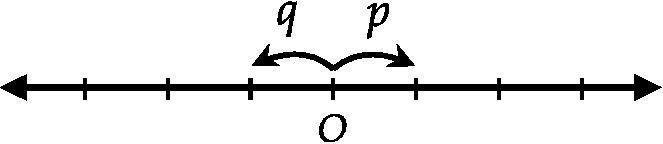
\includegraphics[height=1.5cm,width=8cm]{SP-1}
\end{figure}
\begin{tasks}(4)
\task[\textbf{A.}] $a \sqrt{N p q}$
\task[\textbf{B.}] $a N \sqrt{p q}$
\task[\textbf{C.}] $2 a \sqrt{N p q}$
\task[\textbf{D.}] $a \sqrt{N}$
\end{tasks}
\begin{answer}
\begin{align*}
\text{The standard deviation of Binomial distribution $=\sqrt{N p q}$}\\
\text{Step size } &=2 a\quad (\mathrm{L} \& \mathrm{R})\\
\text{Mean square displacement }&=2 a \sqrt{N p q}
\end{align*}
So the correct answer is \textbf{Option (C)}
\end{answer}
	\item  The rotational energy levels of a molecule are $E_{\ell}=\frac{\hbar^{2}}{2 I_{0}} \ell(\ell+1)$, where $\ell=0,1,2, \ldots$ and $I_{0}$ is its moment of inertia. The contribution of the rotational motion to the Helmholtz free energy per molecule, at low temperatures in a dilute gas of these molecules, is approximately
{	\exyear{NET/JRF(DEC-2018)}}
\begin{tasks}(2)
\task[\textbf{A.}]  $-k_{B} T\left(1+\frac{\hbar^{2}}{I_{0} k_{B} T}\right)$
\task[\textbf{B.}] $-k_{B} T e^{\frac{\hbar^{2}}{I_{0} k_{B} T}}$
\task[\textbf{C.}] $-k_{B} T$
\task[\textbf{D.}] $-3 k_{B} T e^{-\frac{\hbar^{2}}{I_{0} k_{B} T}}$
\end{tasks}
\begin{answer}
\begin{align*}
E_{\ell}&=\frac{\hbar^{2}}{2 I_{0}} \ell(\ell+1) \quad \ell=0,1,2, \ldots\\
z&=\sum_{\ell=0}^{\infty}(2 \ell+1) e^{\frac{-\beta \hbar^{2} \ell(\ell+1)}{2 I_{0}}}\\
z&=1+\sum_{\ell=0}^{\infty}(2 \ell+1) e^{\frac{-\hbar^{2} \ell(\ell+1)}{2 I_{0} k_{B} T}}\\
F&=-k_{B} T \ln z=-k_{B} T \ln \left(1+\sum_{\ell=1}^{\infty}(2 \ell+1) e^{\frac{-\hbar^{2} \ell(\ell+1)}{2 I_{0} k_{B} T}}\right)\\
\ln (1+x)&=x-\frac{x^{2}}{2}+\ldots
\intertext{For low temperature, higher temperature can be neglected}
F&=-k_{B} T \sum_{\ell=1}^{\infty}(2 \ell+1) e^{-\frac{-\hbar^{2} \ell(\ell+1)}{2 I_{0} k_{B} T}}\\&=-k_{B} T\left[3 e^{\frac{-\hbar^{2}}{I_{0} k_{B} T}}+\ldots\right]=-3 k_{B} T e^{-\frac{\hbar^{2}}{I_{0} k_{B} T}}
\end{align*}
So the correct answer is \textbf{Option (D)}
\end{answer}
	\item In a system of $N$ distinguishable particles, each particle can be in one of two states with energies 0 and $-E$, respectively. The mean energy of the system at temperature $T$ is
{	\exyear{NET/JRF(JUNE-2018)}}
\begin{tasks}(2)
\task[\textbf{A.}] $-\frac{1}{2} N\left(1+e^{\varepsilon / k_{B} T}\right)$
\task[\textbf{B.}] $-N E\left(1+e^{\delta / k_{B} T}\right)$
\task[\textbf{C.}] $-\frac{1}{2} N E$
\task[\textbf{D.}] $-N E\left(1+e^{-\delta / k_{B} T}\right)$
\end{tasks}
\begin{answer}
\begin{align*}
\intertext{For one particle system}
\langle E\rangle&=\frac{0 \times e^{\frac{-0}{k_{B} T}}+(-E) e^{+E / k_{B} T}}{e^{-0 / k_{B} T}+e^{E / k_{B} T}}=\frac{-E e^{E / k_{B} T}}{1+e^{E / k_{B} T}}\\&=\frac{-E}{e^{-E / k_{k} T}+1}\langle E\rangle=\frac{-N E}{1+e^{-E / k_{B} T}}
\end{align*}
So the correct answer is \textbf{Option (D)}
\end{answer}
	\item The number of ways of distributing 11 indistinguishable bosons in 3 different energy levels is
	{\exyear{NET/JRF(JUNE-2018)}}
\begin{tasks}(4)
\task[\textbf{A.}]  $3^{11}$
\task[\textbf{B.}] $11^{3}$
\task[\textbf{C.}] $\frac{(13) !}{2 !(11) !}$
\task[\textbf{D.}]  $\frac{(11) !}{3 ! 8 !}$
\end{tasks}
\begin{answer}
\begin{align*}
n&=11 \quad g=3\\
\color{red}\text{answer not completed}
\end{align*}
So the correct answer is \textbf{Option (C)}
\end{answer}
	\item Partition function for a gas of photons is given as, $\ln Z=\frac{\pi^{2} V\left(k_{B} T\right)^{3}}{45 \hbar^{3} C^{3}}$. The specific heat of the photon gas varies with temperature as
{	\exyear{GATE 2010}}
\begin{tasks}(2)
\task[\textbf{A.}] \begin{figure}[H]
	\centering
	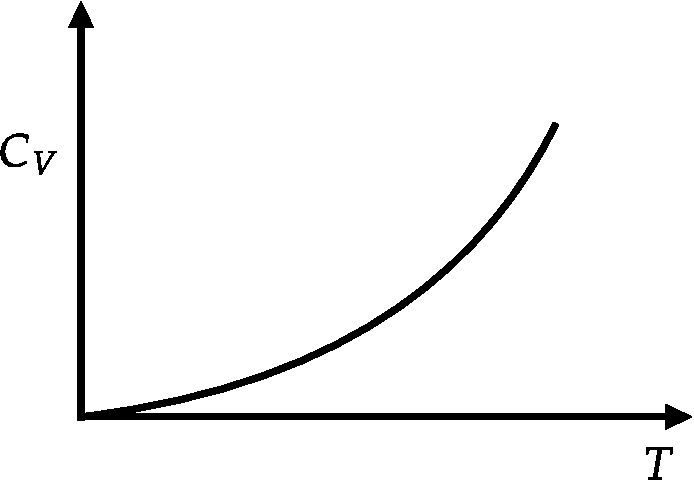
\includegraphics[height=3cm,width=4.5cm]{SP-2}
\end{figure}
\task[\textbf{B.}] \begin{figure}[H]
	\centering
	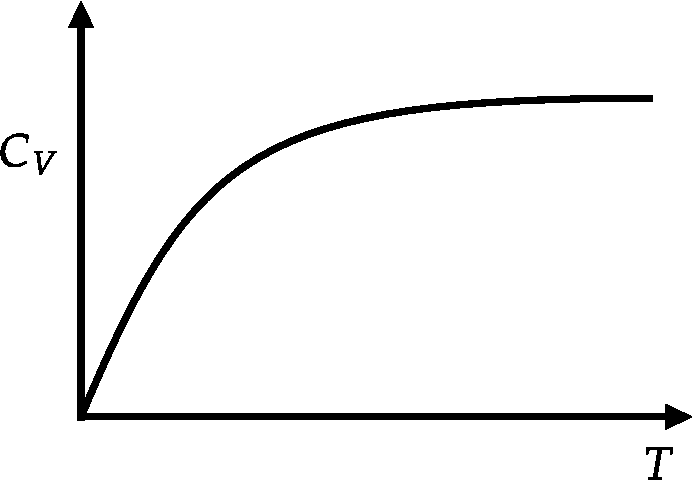
\includegraphics[height=3cm,width=4.5cm]{SP-3}
\end{figure}
\task[\textbf{C.}] \begin{figure}[H]
	\centering
	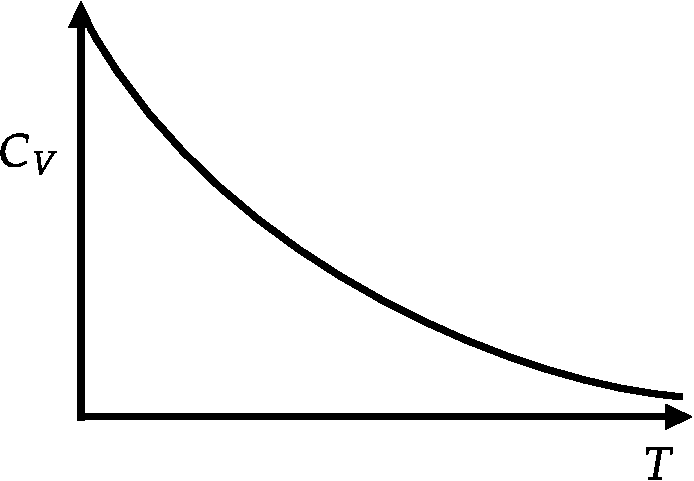
\includegraphics[height=3cm,width=4.5cm]{SP-4}
\end{figure}
\task[\textbf{D.}] \begin{figure}[H]
	\centering
	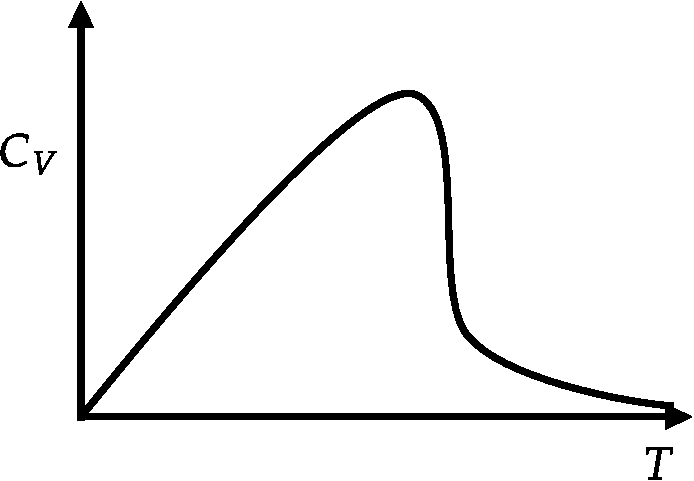
\includegraphics[height=3cm,width=4.5cm]{SP-5}
\end{figure}
\end{tasks}
\begin{answer}
\begin{align*}
\mathrm{U}=\mathrm{K}_{\mathrm{B}} \mathrm{T}^{2} \frac{\partial \ln \mathrm{z}}{\partial \mathrm{T}}, \quad \mathrm{C}_{\mathrm{v}}=\left(\frac{\partial \mathrm{U}}{\partial \mathrm{T}}\right)_{\mathrm{v}} \Rightarrow \mathrm{C}_{\mathrm{v}} \propto \mathrm{T}^{3}
\end{align*}
So the correct answer is \textbf{Option (A)}
\end{answer}
\item 	A system has two energy levels with energies $\varepsilon$ and $2 \varepsilon .$ The lower level is 4 -fold degenerate while the upper level is doubly degenerate. If there are $N$ non-interacting classical particles in the system, which is in thermodynamic equilibrium at a temperature $T$, the fraction of particles in the upper level is
{\exyear{GATE 2011}}
\begin{tasks}(4)
\task[\textbf{A.}] $\frac{1}{1+e^{\varepsilon / k_{B} T}}$
\task[\textbf{B.}] $\frac{1}{1+2 e^{\varepsilon / k_{B} T}}$
\task[\textbf{C.}] $\frac{1}{2 e^{\varepsilon / k_{B} T}+4 e^{2 \varepsilon / k_{B} T}}$
\task[\textbf{D.}] $\frac{1}{2 e^{\varepsilon / k_{B} T}-4 e^{2 \varepsilon / k_{B} T}}$
\end{tasks}
\begin{answer}
\begin{align*}
\text{Partition function }Z&=4 e^{-\epsilon / k T}+2 e^{-\epsilon / k T} \Rightarrow P(2 \varepsilon)\\&=\frac{2 e^{-2 \in / k T}}{4 e^{-\epsilon / k T}+2 e^{-2 \varepsilon / k T}}=\frac{1}{1+2 e^{\epsilon / k T}}
\end{align*}
So the correct answer is \textbf{Option (B)}
\end{answer}
\item 	For an ideal Fermi gas in three dimensions, the electron velocity $V_{F}$ at the Fermi surface is related to electron concentration $n$ as,
{\exyear{GATE 2012}}
\begin{tasks}(4)
\task[\textbf{A.}] $V_{F} \propto n^{2 / 3}$
\task[\textbf{B.}]  $V_{F} \propto n$
\task[\textbf{C.}] $V_{F} \propto n^{1 / 2}$
\task[\textbf{D.}] $V_{F} \propto n^{1 / 3}$
\end{tasks}
\begin{answer}
\begin{align*}
E_{F}&=\frac{1}{2} m V_{F}^{2} \quad \because E_{F} \propto n^{2 / 3} \Rightarrow V_{F}^{2} \propto n^{2 / 3} \Rightarrow V_{F} \propto n^{1 / 3}
\end{align*}
So the correct answer is \textbf{Option (D)}
\end{answer}
	\item Consider a system whose three energy levels are given by $0, \varepsilon$ and $2 \varepsilon$. The energy level $\varepsilon$ is two-fold degenerate and the other two are non-degenerate. The partition function of the system with $\beta=\frac{1}{k_{B} T}$ is given by
{	\exyear{GATE 2012}}
\begin{tasks}(2)
\task[\textbf{A.}] $1+2 e^{-\beta \varepsilon}$
\task[\textbf{B.}] $2 e^{-\beta \varepsilon}+e^{-2 \beta \varepsilon}$
\task[\textbf{C.}] $\left(1+e^{-\beta \varepsilon}\right)^{2}$
\task[\textbf{D.}] $1+e^{-\beta \varepsilon}+e^{-2 \beta \varepsilon}$
\end{tasks}
\begin{answer}
\begin{align*}
E_{1}&=0, E_{2}=\varepsilon, E_{3}=2 \varepsilon ; g_{1}=1, g_{2}=2, g_{3}=1\\&\text{ where} g_{1}, g_{2}\text{ and }g_{3}\text{ are degeneracy}\\
\text{	The partition function }Z&=g_{1} e^{-\beta \cdot E_{1}}+g_{2} e^{-\beta \cdot E_{2}}+g_{3} e^{-\beta \cdot E_{3}}\\&=1+2 e^{-\beta c}+e^{-\beta 2 \varepsilon}=\left(1+e^{-\beta c}\right)^{2}
\end{align*}
\end{answer}
	\item Consider a linear collection of $N$ independent spin $1 / 2$ particles, each at a fixed location. The entropy of this system is $(k$ is the Boltzmann constant)
{	\exyear{GATE 2013}}
\begin{tasks}(4)
\task[\textbf{A.}] Zero
\task[\textbf{B.}]  $N k$
\task[\textbf{C.}]  $\frac{1}{2} N k$
\task[\textbf{D.}] $N k \ln (2)$
\end{tasks}
\begin{answer}
There are two microstates possible for spin $\frac{1}{2}$ particle, so entropy is given by $N k \ln (2)$\\\\
So the correct answer is \textbf{Option (D)}
\end{answer}
	\item Let $N_{M B}, N_{B E}, N_{F D}$ denote the number of ways in which two particles can be distributed in two energy states according to Maxwell-Boltzmann, Bose-Einstein and Fermi-Dirac statistics respectively. Then $N_{M B}: N_{B E}: N_{F D}$ is
	{\exyear{JAM 2013}}
\begin{tasks}(4)
\task[\textbf{A.}]  $4: 3: 1$
\task[\textbf{B.}]  $4: 2: 3$
\task[\textbf{C.}] $4: 3: 3$
\task[\textbf{D.}] $4: 3: 2$
\end{tasks}
\begin{answer}
For Maxwell, Boltzmann, $$W=\frac{\underline{N}}{\lfloor n}$$ $$g^{n}=\frac{[2}{\lfloor 2} 2^{2}=4$$
For Boson, $$N=2, g=2, n=2$$ 
$$ W=\frac{\lfloor n+g-1}{\lfloor\underline{n} \mid g-1}=\frac{\mid 2+2-1}{\lfloor 2 \mid 2-1}=3$$
For Fermion, $$N=2, g=2, n=2$$
$$ W=\frac{\mid g}{|g| g-n}=\frac{\lfloor 2}{\lfloor 2 \mid 1}=1$$
Correct answer is \textbf{option (A)}
\end{answer}
\item In 1 - dimension, an ensemble of $N$ classical particles has energy of the form $E=\frac{P_{x}^{2}}{2 m}+\frac{1}{2} k x^{2}$. The average internal energy of the system at temperature $T$ is 
{\exyear{JAM 2014}}
\begin{tasks}(4)
\task[\textbf{A.}] $\frac{3}{2} N k_{B} T$
\task[\textbf{B.}] $\frac{1}{2} N k_{B} T$ 
\task[\textbf{C.}] $3 N k_{B} T$
\task[\textbf{D.}] $N k_{B} T$
\end{tasks}
\begin{answer}
Since, $E=\left(\frac{P_{x}^{2}}{2 m}+\frac{1}{2} k x^{2}\right)$\\
Now, $\langle E\rangle=\frac{1}{2 m}\left\langle P_{x}^{2}\right\rangle+\frac{1}{2} k\left\langle x^{2}\right\rangle=\frac{k T}{2}+\frac{k T}{2}=k T$\\
And for $N$ - classical particle, $\langle E\rangle=N k T$\\
Correct answer is \textbf{option ()}
\end{answer}	
	\item A system consists of $N$ number of particles, $N>1 .$ Each particle can have only one of the two energies $E_{1}$ or $E_{1}+\varepsilon(\varepsilon>0) .$ If the system is in equilibrium at a temperature $T$ the average number of particles with energy $E_{1}$ is
{	\exyear{JAM 2015}}
\begin{tasks}(4)
\task[\textbf{A.}] $\frac{N}{2}$
\task[\textbf{B.}] $\frac{N}{e^{\delta / k T}+1}$ 
\task[\textbf{C.}] $\frac{N}{e^{-\varepsilon / k T}+1}$
\task[\textbf{D.}] $N e^{-\delta / k T}$
\end{tasks}
\begin{answer}
$\langle N\rangle=N e^{\frac{-\left(E_{2}-E_{1}\right)}{k T}}$\\
$=N e^{\frac{-\left[\left(E_{1}+\varepsilon\right)-E_{1}\right]}{k T}} \Rightarrow\langle N\rangle=N e^{\frac{-\varepsilon}{k T}}$\\
Correct answer is \textbf{option (D)}
\end{answer}
	
	
	
	
	
	
	
	
	
	
	
	
	
	
	
	
	
	
\end{enumerate}